%%%%%%%%%%%%%%%%%%%%%%%%%%%%%%%%%%%%%%%%%
% Beamer Presentation
% LaTeX Template
% Version 1.0 (10/11/12)
%
% This template has been downloaded from:
% http://www.LaTeXTemplates.com
%
% License:
% CC BY-NC-SA 3.0 (http://creativecommons.org/licenses/by-nc-sa/3.0/)
%
%%%%%%%%%%%%%%%%%%%%%%%%%%%%%%%%%%%%%%%%%

%----------------------------------------------------------------------------------------
%	PACKAGES AND THEMES
%----------------------------------------------------------------------------------------

\documentclass{beamer}

\mode<presentation>{% The Beamer class comes with a number of default slide themes
% which change the colors and layouts of slides. Below this is a list
% of all the themes, uncomment each in turn to see what they look like.

%\usetheme{default}
%\usetheme{AnnArbor}
%\usetheme{Antibes}
%\usetheme{Bergen}
%\usetheme{Berkeley}
\usetheme[compress]{Berlin}
%\usetheme{Boadilla}
%\usetheme{CambridgeUS}
%\usetheme{Copenhagen}
%\usetheme{Darmstadt}
%\usetheme{Dresden}
%\usetheme{Frankfurt}
%\usetheme{Goettingen}
%\usetheme{Hannover}
%\usetheme{Ilmenau}
%\usetheme{JuanLesPins}
%\usetheme{Luebeck}
%\usetheme{Madrid}
%\usetheme{Malmoe}
%\usetheme{Marburg}
%\usetheme{Montpellier}
%\usetheme{PaloAlto}
%\usetheme{Pittsburgh}
%\usetheme{Rochester}
%\usetheme{Singapore}
%\usetheme{Szeged}
%\usetheme{Warsaw}

% As well as themes, the Beamer class has a number of color themes
% for any slide theme. Uncomment each of these in turn to see how it
% changes the colors of your current slide theme.

%\usecolortheme{albatross}
%\usecolortheme{beaver}
%\usecolortheme{beetle}
%\usecolortheme{crane}
%\usecolortheme{dolphin}
%\usecolortheme{dove}
%\usecolortheme{fly}
%\usecolortheme{lily}
%\usecolortheme{orchid}
%\usecolortheme{rose}
%\usecolortheme{seagull}
%\usecolortheme{seahorse}
%\usecolortheme{whale}
%\usecolortheme{wolverine}

\makeatother
\setbeamertemplate{footline}
{
  \leavevmode%
  \hbox{%
  \begin{beamercolorbox}[wd=.3\paperwidth,ht=2.25ex,dp=1ex,center]{section in head/foot}%
    \usebeamerfont{author in head/foot}\insertshortauthor
  \end{beamercolorbox}%
  \begin{beamercolorbox}[wd=.6\paperwidth,ht=2.25ex,dp=1ex,center]{subsection in head/foot}%
    \usebeamerfont{title in head/foot}\insertshorttitle
  \end{beamercolorbox}%
  \begin{beamercolorbox}[wd=.1\paperwidth,ht=2.25ex,dp=1ex,center]{title}%
    \usebeamerfont{instritute in head/foot}\insertshortinstitute
  \end{beamercolorbox}}%
  \vskip0pt%
}
\makeatletter

%\setbeamertemplate{footline} % To remove the footer line in all slides uncomment this line
%\setbeamertemplate{footline}[page number] % To replace the footer line in all slides with a simple slide count uncomment this line

\setbeamertemplate{navigation symbols}{} % To remove the navigation symbols from the bottom of all slides uncomment this line
}

\usepackage[english]{babel} 
\usepackage[utf8]{inputenc}

\usepackage{graphicx} % Allows including images
\usepackage{caption}
\usepackage{booktabs} % Allows the use of \toprule, \midrule and \bottomrule in tables
\usepackage{multicol} 

% Math packages
\usepackage{amsmath}
\usepackage{mathtools}
\usepackage{amssymb}
\usepackage{mathpartir}

%----------------------------------------------------------------------------------------
%	TITLE PAGE
%----------------------------------------------------------------------------------------

\title[Mathematical Foundations and the Foundational Crisis]{Foundations of Mathematics\\and the Foundational Crisis} % The short title appears at the bottom of every slide, the full title is only on the title page

\author{Kevin Kappelmann} % Your name
\institute[TUM] % Your institution as it will appear on the bottom of every slide, may be shorthand to save space
{Technical University of Munich}
\date{\today} % Date, can be changed to a custom date

\begin{document}

\begin{frame}
\titlepage % Print the title page as the first slide
\end{frame}

%----------------------------------------------------------------------------------------
%	PRESENTATION SLIDES
%----------------------------------------------------------------------------------------
%\section*{Introduction}
%------------------------------------------------
%\begin{frame}
    %\frametitle{}
    %\begin{itemize}[<+->]
	%\item Mathematics strives for absolute certainty.
	%\item For this, we use rigorous proofs.
	%\item When shall I accept a proof?
	%\item Can we trust each other?
	%\item Can we trust a computer?
	%\begin{itemize}
		%\item Computer-generated proofs are barely verifiable by hand.
		%\item[$\Rightarrow$] Controversies
	%\end{itemize}
	%\item But it is not the first controversy in mathematical history\ldots
    %\end{itemize}
%\end{frame}
%------------------------------------------------
% Overview slide
%------------------------------------------------
\begin{frame}
    \frametitle{Overview} 
    %\begin{multicols}{2}
        \tableofcontents
    %\end{multicols}
\end{frame}
%------------------------------------------------
\section{Causes of the crisis}
%------------------------------------------------
\subsection{Ancient Mathematics}
%------------------------------------------------
\begin{frame}
    \frametitle{First Steps}
    \begin{itemize}[<+->]
	\item In the beginning, maths served as an applied tool.
	\item Ancient Greeks developed the notion of a proof in 600 BC.
	\item The Pythagoreans discovered irrational numbers.
	\begin{itemize}
		\item[$\Rightarrow$] First controversy of mathematics
	\end{itemize}
	\item Euclid's Elements around 300 BC
	\begin{itemize}
		\item Axiomatic, deductive treatment of mathematics similar to modern systems
		\item A work of timeless certainty\ldots\\\uncover<+->{\ldots at least so had been thought}
	\end{itemize}
    \end{itemize}
\end{frame}
\begin{frame}
    \frametitle{Euclid's Postulates}
	``Let the following be postulated:\pause
     \begin{enumerate}[<+->]
	\item To draw a straight line from any point to any point.
	\item To produce [extend] a finite straight line continuously in a straight line.
	\item To describe a circle with any centre and distance [radius].
	\item That all right angles are equal to one another.
	\item That, if a straight line falling on two straight lines make the interior angles on the same side less than two right angles, the two straight lines, if produced indefinitely, meet on that side on which are the angles less than the two right angles.''
     \end{enumerate}
\end{frame}
%------------------------------------------------
\subsection{Uncertainties}
%------------------------------------------------
\begin{frame}
    \frametitle{Search for Foundations}
    \begin{itemize}[<+->]
	\item Gauß proved the independence of Euclid's fifth postulate in 1813.
	\begin{itemize}
		\item[$\Rightarrow$] Scepticism towards used systems
	\end{itemize}
	\item Rigorous axiomatisation of mathematical branches in the late 19th century
	\begin{itemize}
		\item Arithmetic of natural numbers by Peano
		\item<.-> Geometry by Hilbert and Pasch
		\item<.-> Predicate logic by Frege
	\end{itemize}
	\item Desire for a universal and consistent system
    \end{itemize}
\end{frame}
\begin{frame}
    \frametitle{Universal Systems}
    \begin{itemize}[<+->]
	\item Cantor's set theory
	\begin{itemize}
		\item \textit{``A set is a gathering together into a whole of definite, distinct objects of our perception or of our thought --- which are called elements of the set.''}\nocite{cantor_set}\hfill--- Georg Cantor
		\item Certainly universal, but informal and thus not adequate for a study of consistency
		\item Nonetheless, it was widely accepted.
	\end{itemize}
	\item Frege tried to build a consistent foundation with logic.
	\begin{itemize}
		\item<.-> Sophisticated work, but not well received
	\end{itemize}
	\item And then came Russell\ldots
    \end{itemize}
\end{frame}
\begin{frame}
    \frametitle{Russell's Paradox}
	Consider \textit{the set of all sets that are not members of themselves}:
	\begin{equation*}
		R\coloneqq\{X\mid X\notin X\}
	\end{equation*}\pause
	Question: Is R a member of itself? That is, does $R\in R$ hold?\pause\\
	\vspace{\baselineskip}
	Answer:\hspace{4.3em}$R\in R \iff R\notin R$, a contradiction!
\end{frame}
\begin{frame}
    \frametitle{The Begin of the Crisis}
    \begin{itemize}[<+->]
	\item Cantor's as well as Frege's system were victims of this paradox.
	\item \textit{``Hardly anything more unfortunate can befall a scientific writer than to have one of the foundations of his edifice shaken after the work is finished.''\nocite{frege_appendix}}\hfill--- Gottlob Frege
	\item Systems founded on Cantor's set theory were on shaky ground.
	\item A new foundation of mathematics had to be found.
    \end{itemize}
\end{frame}
%------------------------------------------------
\section{The Foundational Crisis}
\begin{frame}
    \frametitle{The Three Schools of Thought}
    \begin{itemize}[<+->]
	\item Three schools of thought tried to establish a new foundation.
	\begin{itemize}
		\item<.-> Logicism
		\item<.-> Intuitionism
		\item<.-> Formalism
	\end{itemize}
    \end{itemize}
\centering{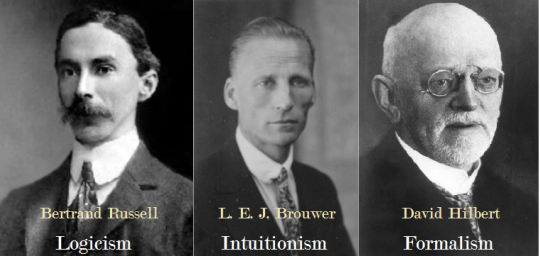
\includegraphics[height=0.42\textheight]{img/logic_intuit_form.png}\\
\scriptsize{Source: \url{geopolicraticus.tumblr.com/post/142561195372}}}
\end{frame}
%------------------------------------------------
\subsection{Logicism}
\begin{frame}
    \frametitle{A Foundation Made of Logic}
    \begin{itemize}[<+->]
	\item Russell and Whitehead revisited the idea of reducing mathematics to logic, as tried by Frege.	
	\item Mathematics as an extension of logic
	\item Only few axioms that must pose fundamental logical principles 
	\item Chief work: Principia Mathematica
    \end{itemize}
\end{frame}
\begin{frame}
    \frametitle{Principia Mathematica}
    \only<1-4>{
    \begin{itemize}[<+->]
	\item Type theory to avoid antinomies
	\item Difficulties in explaining some axioms
	\begin{itemize}
		\item<.-> Axiom of reducibility
		\item<.-> Axiom of infinity
	\end{itemize}
	\item Regarded as ``the outstanding example of an unreadable masterpiece.''\nocite{math_experience}
	\item Nonetheless, many adopted it as a new foundation.
    \end{itemize}}
    \only<5>{
	    \begin{centering}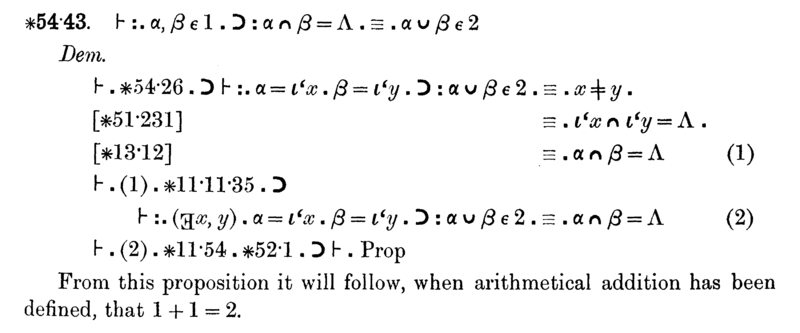
\includegraphics[width=\textwidth]{img/principia_mathematica.png}\end{centering}\\
	    \scriptsize{Principia Mathematica's infamous proof of $1+1=2$. It was not until page 379 that this proof was possible.}
    }
\end{frame}
%------------------------------------------------
\subsection{Intuitionism}
\begin{frame}
    \frametitle{Proofs with Real Evidence}
    \begin{itemize}[<+->]
	\item Mathematics is \textbf{not} reducible to some formal system.
	\item Mathematics is a constructive process conducted by humans.
	\item The existence of any mathematical object ist equivalent to the possibility of its construction, according to Brouwer.
	\begin{itemize}
		\item[$\Rightarrow$] No antinomies as paradoxical sets cannot be constructed.
	\end{itemize}
	\item Consequently, some assumptions of classical logic must be rejected.
    \end{itemize}
\end{frame}
\begin{frame}
    \frametitle{$P\lor\lnot P\equiv\ $?}
    \begin{itemize}[<+->]
	\item Intuitionists reject the \textit{law of excluded middle}: $\vdash P\lor\lnot P$\\
		\begin{centering}
			``For any proposition P, either P or its negation is true.''
		\end{centering}
    \end{itemize}
	\pause[\thebeamerpauses]
	\textbf{Proposition:} There exist two irrational numbers $a$ and $b$ such that $a^b$ is rational.\\\pause
	\vspace{\baselineskip}
	\textbf{Proof.} It is known that $\sqrt{2}$ is irrational. Let us consider the number $\sqrt{2}^{\sqrt{2}}$.\pause$ $ If it is rational, our statement is proved.\pause$ $ If it is irrational, $(\sqrt{2}^{\sqrt{2}})^{\sqrt{2}}=2$ proves our statement.\hfill$\qed$
\end{frame}
\begin{frame}
    \frametitle{The Price to Pay}
    \begin{itemize}[<+->]
	\item Intuitionistic logic aggravates many proofs.
	\item \textit{``Taking this tertium non datur (law of excluded middle) from the mathematician would be the same as, say, denying the astronomer his telescope and the boxer the use of his fists.''}\nocite{hilbert_tertium_non_datur}\\\hfill--- David Hilbert
	\item Consequently, only a few scholars adhered to intuitionism.
    \end{itemize}
\end{frame}
%------------------------------------------------
\subsection{Formalism}
\begin{frame}
    \frametitle{Mathematics as a Symbol Modifier}
    \begin{itemize}[<+->]
	\item Formalists support the autonomy of mathematics.
	\item Mathematics shall be based on symbols and axioms that describe syntactical operations on them.
	\item Mathematics must not justify the existence of its objects as its objects are just meaningless shapes.
    \end{itemize}
\end{frame}
\begin{frame}
    \frametitle{Hilbert's Dream}
    \begin{itemize}[<+->]
	\item Hilbert feared the crippling effect of intuitionistic logic.
	\item To save mathematics, he initiated a research programme called \textit{Hilbert's program} consistings of two steps:
	\begin{enumerate}
		\item Formalise a system that is able to derive all of mathematics using syntactical operations.
		\item Prove the system's consistency with metamathematical reasoning.
	\end{enumerate}
	\item The dream of a complete and consistent mathematical system
	\item However, this dream just stayed a dream\ldots
    \end{itemize}
\end{frame}
%------------------------------------------------
\subsection{Peak and End}
\begin{frame}
    \frametitle{The Peak of the Crisis}
    \begin{itemize}[<+->]
	\item In 1928, Brouwer boycotted the International Congress of Mathematicians.
	\item There he presented his programme, without Brouwer being able to descredit his ideas.
	\item A few days after, Hilbert excluded Brouwer as a co-publisher from the journal ``Mathematischen Annalen''.
	\item Brouwer, in a state of frustration and despair, subsequently stopped publishing intuitionistic articles.
	\item Optimism for a complete and consistent formal system grew\ldots
    \end{itemize}
\end{frame}
\begin{frame}
    \frametitle{The End of the Crisis}
\begin{columns}
 \begin{column}{.49\textwidth}
    \begin{itemize}[<+->]
	\item \ldots but then came Gödel.
	\item In 1931, he proved that there is no sufficiently strong, complete and consistent formal system.
    \end{itemize}
 \end{column}
 \begin{column}{.49\textwidth}
  \centering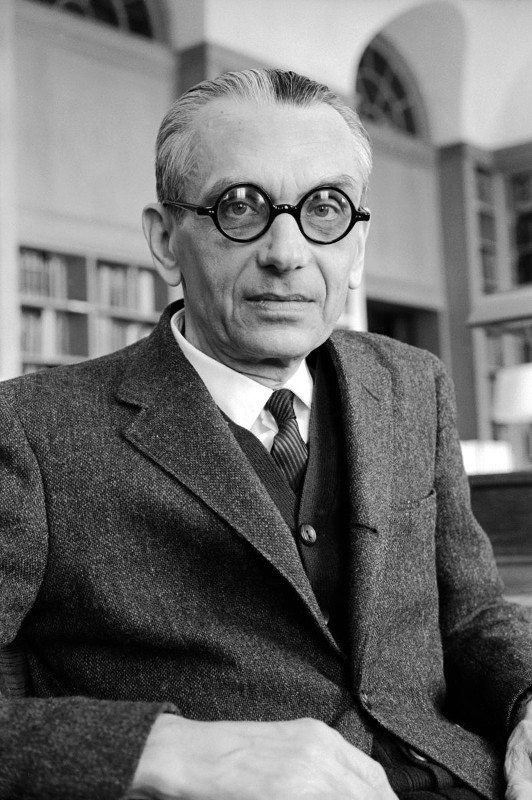
\includegraphics[height=0.35\textheight]{img/goedel.jpg}\\
		\scriptsize{Source: \url{newyorker.com/tech/elements/waiting-for-godel}}
 \end{column}
\end{columns}
    \visible<3>{\begin{theorem}[Second Incompleteness Theorem] Any consistent formal system rich enough to contain a formalisation of recursive arithmetic cannot prove its own consistency.\end{theorem}}
\end{frame}
%------------------------------------------------
\section{Aftermath and Prospects}
\begin{frame}
    \frametitle{Modern Mathematics}
    \begin{itemize}[<+->]
	\item In 1928, Brouwer boycotted the International Congress of Mathematicians.
	\item There he presented his programme, without Brouwer being able to descredit his ideas.
	\item A few days after, Hilbert excluded Brouwer as a co-publisher from the journal ``Mathematischen Annalen''.
	\item Brouwer, in a state of frustration and despair, subsequently stopped publishing intuitionistic articles.
	\item Optimism for a complete and consistent formal system grew\ldots
    \end{itemize}
\end{frame}
%------------------------------------------------
\section*{}
%------------------------------------------------
\begin{frame}
    \Huge{\centerline{The End}}
\end{frame}
%----------------------------------------------------------------------------------------

\newpage
\bibliographystyle{plain}
\bibliography{../../paper/sources.bib}
\end{document} 
